\documentclass[12pt]{article}\usepackage[]{graphicx}\usepackage[]{color}
%% maxwidth is the original width if it is less than linewidth
%% otherwise use linewidth (to make sure the graphics do not exceed the margin)
\makeatletter
\def\maxwidth{ %
  \ifdim\Gin@nat@width>\linewidth
    \linewidth
  \else
    \Gin@nat@width
  \fi
}
\makeatother

\definecolor{fgcolor}{rgb}{0.345, 0.345, 0.345}
\newcommand{\hlnum}[1]{\textcolor[rgb]{0.686,0.059,0.569}{#1}}%
\newcommand{\hlstr}[1]{\textcolor[rgb]{0.192,0.494,0.8}{#1}}%
\newcommand{\hlcom}[1]{\textcolor[rgb]{0.678,0.584,0.686}{\textit{#1}}}%
\newcommand{\hlopt}[1]{\textcolor[rgb]{0,0,0}{#1}}%
\newcommand{\hlstd}[1]{\textcolor[rgb]{0.345,0.345,0.345}{#1}}%
\newcommand{\hlkwa}[1]{\textcolor[rgb]{0.161,0.373,0.58}{\textbf{#1}}}%
\newcommand{\hlkwb}[1]{\textcolor[rgb]{0.69,0.353,0.396}{#1}}%
\newcommand{\hlkwc}[1]{\textcolor[rgb]{0.333,0.667,0.333}{#1}}%
\newcommand{\hlkwd}[1]{\textcolor[rgb]{0.737,0.353,0.396}{\textbf{#1}}}%

\usepackage{framed}
\makeatletter
\newenvironment{kframe}{%
 \def\at@end@of@kframe{}%
 \ifinner\ifhmode%
  \def\at@end@of@kframe{\end{minipage}}%
  \begin{minipage}{\columnwidth}%
 \fi\fi%
 \def\FrameCommand##1{\hskip\@totalleftmargin \hskip-\fboxsep
 \colorbox{shadecolor}{##1}\hskip-\fboxsep
     % There is no \\@totalrightmargin, so:
     \hskip-\linewidth \hskip-\@totalleftmargin \hskip\columnwidth}%
 \MakeFramed {\advance\hsize-\width
   \@totalleftmargin\z@ \linewidth\hsize
   \@setminipage}}%
 {\par\unskip\endMakeFramed%
 \at@end@of@kframe}
\makeatother

\definecolor{shadecolor}{rgb}{.97, .97, .97}
\definecolor{messagecolor}{rgb}{0, 0, 0}
\definecolor{warningcolor}{rgb}{1, 0, 1}
\definecolor{errorcolor}{rgb}{1, 0, 0}
\newenvironment{knitrout}{}{} % an empty environment to be redefined in TeX

\usepackage{alltt}
\usepackage{graphicx}
\usepackage{verbatim}
\usepackage{pdfpages}
\usepackage{float}
\setlength{\topmargin}{-.8 in}
\setlength{\textheight}{9.4  in}
\setlength{\oddsidemargin}{-.1in}
\setlength{\evensidemargin}{-.1in}
\setlength{\textwidth}{6.35in}
\include{macros}
\IfFileExists{upquote.sty}{\usepackage{upquote}}{}
\begin{document}



\begin{center}
{\bf Effective Sample Size $\hat{n}_{eff}$}\\
Garland Will \& Leslie Gains-Germain \& Matt Tyers\\
\end{center}

\noindent In Bayesian Data Analysis 3 by Gelman, et.al. effective sample size is calculated as

$$\hat{n}_{eff} = \frac{mn}{1 + 2 \sum_{t=1}^{T}\widehat{\rho_t}}; \hspace{.5 in} \widehat{\rho_t} = 1- \frac{V_t}{2 \widehat{var}^+}$$

\noindent In the above formula, $\widehat{var}^+$ is the marginal posterior variance, and is a weighted average of the between and within chain variance. M is the number of chains and n is the the number of draws from each chain.  $V_t$ is the variogram at each lag, where smaller $V_t$ values indicate higher correlation. \\  


\noindent Calculation of the effective sample size $\hat{n}_{neff}$ in coda is done using a different (and much more code-efficient) technique than the algorithm presented in Chapter 11 of the Gelman, et.al. text. Function effectiveSize() first checks to see if it has been passed an MCMC list. If so, it breaks the list apart by variables and runs itself on the set of chains for each variable. Otherwise (or after this), it calls \verb+spectrum0.ar()+ to calculate the spectral density at frequency zero of each chain.  \verb+Spectrum0.ar()+ fits an autoregressive model to the chain, treating the chain as a time series. %The spectral density at frequency zero is found by using a fast fourier transform and then fitting a glm model to the chain. 
The larger the variance left unexplained by the autoregressive model, the larger the spectral density at frequency zero, reflecting higher correlation within the chain. \\

%and then divides this by the length of the chain to estimate the variance of the mean.

%The spectral density spec is calculated in spectrum0.ar() as

%$$spec = \frac{Variance.unexplained.by.autoregressive.model}{(1 - \sum{AutoRegressive.coefficients)^2}}$$


\noindent If the spectral density is zero, i.e. there is no variance in the chain left unexplained by the autoregressive model, \verb+effectiveSize+ returns an effective sample size of $\hat{n}_{neff} = 0$ for the chain. If not, it returns

$$\hat{n}_{eff} = \sum_{i=1}^{K}\frac{number.of.iterations * V(chain_i)}{spec_i}$$

\noindent Where $V(chain_i)$ is the overall variance of chain $i$, $spec_i$ is the spectral density as described above for the $i$th chain, and $K$ is the number of chains. \\

\noindent {\bf Somewhat worrisome example} \\
\noindent This example looks at simulating three chains of length 1,000 from a multivariate normal.  All of the chains have a mean of 0, and correlation equal to 0.8.  Looking at the traceplots, the three chains are very correlated with one another.  Using the coda package to calculate effective sample size on each chain, we get values above 1,000 which is the number of draws for each chain. This serves as an illustration that n effective as calculated in coda is not a perfect diagnostic tool, as having an effective sample size greater than the number of draws is not reasonable.  Also worth noting is that coda calculates n effective strictly within each chain.  The method from the BDA3 on the other hand uses a variance that is a weighted average of the between and within chain variance.  
\begin{knitrout}
\definecolor{shadecolor}{rgb}{0.969, 0.969, 0.969}\color{fgcolor}\begin{kframe}
\begin{alltt}
\hlkwd{set.seed}\hlstd{(}\hlnum{38}\hlstd{)}
\hlkwd{require}\hlstd{(coda,} \hlkwc{quietly} \hlstd{= T)}
\hlkwd{require}\hlstd{(mvtnorm,} \hlkwc{quietly} \hlstd{= T)}
\hlstd{d} \hlkwb{<-} \hlkwd{matrix}\hlstd{(}\hlkwd{c}\hlstd{(}\hlnum{1}\hlstd{,} \hlnum{0}\hlstd{,} \hlnum{0}\hlstd{,} \hlnum{0}\hlstd{,} \hlnum{1}\hlstd{,} \hlnum{0}\hlstd{,} \hlnum{0}\hlstd{,} \hlnum{0}\hlstd{,} \hlnum{1}\hlstd{),} \hlkwc{nrow} \hlstd{=} \hlnum{3}\hlstd{,} \hlkwc{ncol} \hlstd{=} \hlnum{3}\hlstd{)}
\hlstd{r} \hlkwb{<-} \hlkwd{matrix}\hlstd{(}\hlkwd{c}\hlstd{(}\hlnum{1}\hlstd{,} \hlnum{0.8}\hlstd{,} \hlnum{0.8}\hlstd{,} \hlnum{0.8}\hlstd{,} \hlnum{1}\hlstd{,} \hlnum{0.8}\hlstd{,} \hlnum{0.8}\hlstd{,} \hlnum{0.8}\hlstd{,} \hlnum{1}\hlstd{),} \hlkwc{nrow} \hlstd{=} \hlnum{3}\hlstd{,} \hlkwc{ncol} \hlstd{=} \hlnum{3}\hlstd{)}
\hlstd{v} \hlkwb{<-} \hlstd{d} \hlopt \hlstd{r} \hlopt \hlstd{d}
\hlstd{chains} \hlkwb{<-} \hlkwd{rmvnorm}\hlstd{(}\hlnum{1000}\hlstd{,} \hlkwd{c}\hlstd{(}\hlnum{0}\hlstd{,} \hlnum{0}\hlstd{,} \hlnum{0}\hlstd{),} \hlkwc{sigma} \hlstd{=} \hlkwd{sqrt}\hlstd{(v))}
\end{alltt}
\end{kframe}
\end{knitrout}

\begin{knitrout}
\definecolor{shadecolor}{rgb}{0.969, 0.969, 0.969}\color{fgcolor}

{\centering 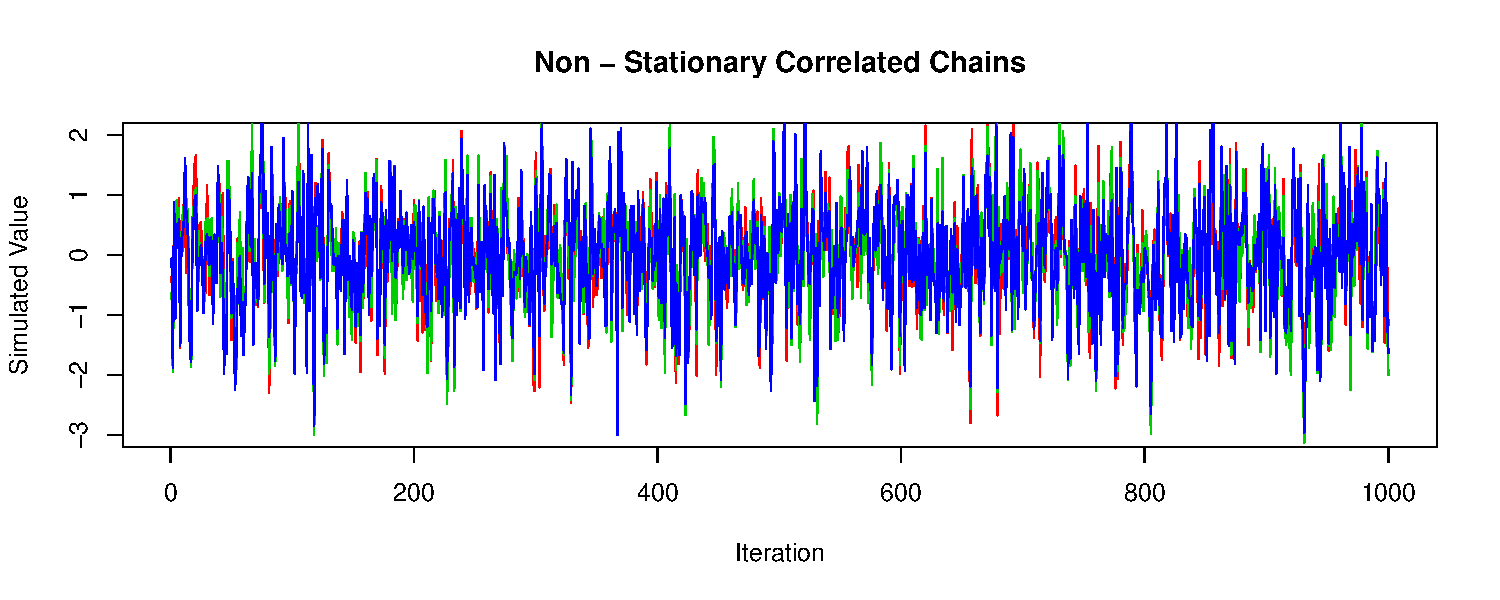
\includegraphics[width=\linewidth]{figure/plots-1} 

}



\end{knitrout}

% latex table generated in R 3.2.2 by xtable 1.7-4 package
% Tue Nov 17 11:51:18 2015
\begin{table}[H]
\centering
\caption{Effective sample size} 
\begin{tabular}{rr}
  \hline
 & Effective Sample Size \\ 
  \hline
Chain 1 & 1443.15 \\ 
  Chain 2 & 1210.35 \\ 
  Chain 3 & 1000.00 \\ 
   \hline
\end{tabular}
\end{table}

\end{document}
